\scanpage{110}
% archive foliation: 109
a) Donnons-nous un idéal $R\subset B$. Alors

Décomposition de $\unsure{B|A}/R$ en produit de deux anneaux
\[
\simeq\ \text{Donnée de deux idéaux }J,J'\text{ de }A\text{ tels que}
\]
\[
JJ'=R,\quad J+J'=A
\]
\margin{[Car $J+J'=A\Rightarrow JJ'=J\cap J'$]}

b) Supposons $B=A[T]$, \inserted{\figure{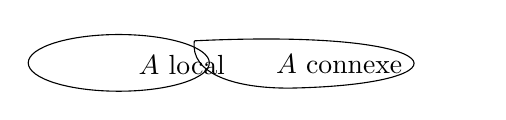
\begin{tikzpicture}
\node at (0,0) {\deleted{$A$ \uline{local}}};
\node at (2.0,0) {$A$ connexe};
\draw (-0.8,0.02) ellipse (1.15 and 0.36);
\draw (0.16,0.30) .. controls (3.5,0.46) and (3.75,-0.25) .. (1.40,-0.30)
 .. controls (0.68,-0.31) and (0.10,-0.12) .. (0.16,0.30);
\end{tikzpicture}}} $R=(P)$, $P$ polynôme \uline{unitaire}, Alors tte décomposition de $R$ en produit de deux idéaux $J,J'$ tels que $J+J'=B$, est \unsure{uniquement} de la forme $(\unsure{P|R})=(Q)(Q')$, où $Q,Q'$ sont des polynômes \uline{unitaires} tels que
\[
P=QQ'.
\]

Si elle est donnée par une telle déc., alors $P$ est unique à une unité près, et tt \unsure{repr.} unitaire est unique
\deleted{[\unsure{NB.}\quad\unsure{faut}}
[petite vérification\ldots]. \deleted{On}
\deleted{\unsure{prouver que}} \deleted{On}
\unsure{l'unicité résulte qu'} l'on peut supposer $\unsure{\operatorname{Spec}} A$ \uline{local}. Alors pour l'existence, on voit que c'est vrai sur les
